\atsptt
    \begin{frame}{\ft{Link and Dependency Grammar Annotations}}
\section{Group 2: Link and Dependency Grammar Annotations}

        \begin{annotatedFigure}{0pt}{0pt}
            {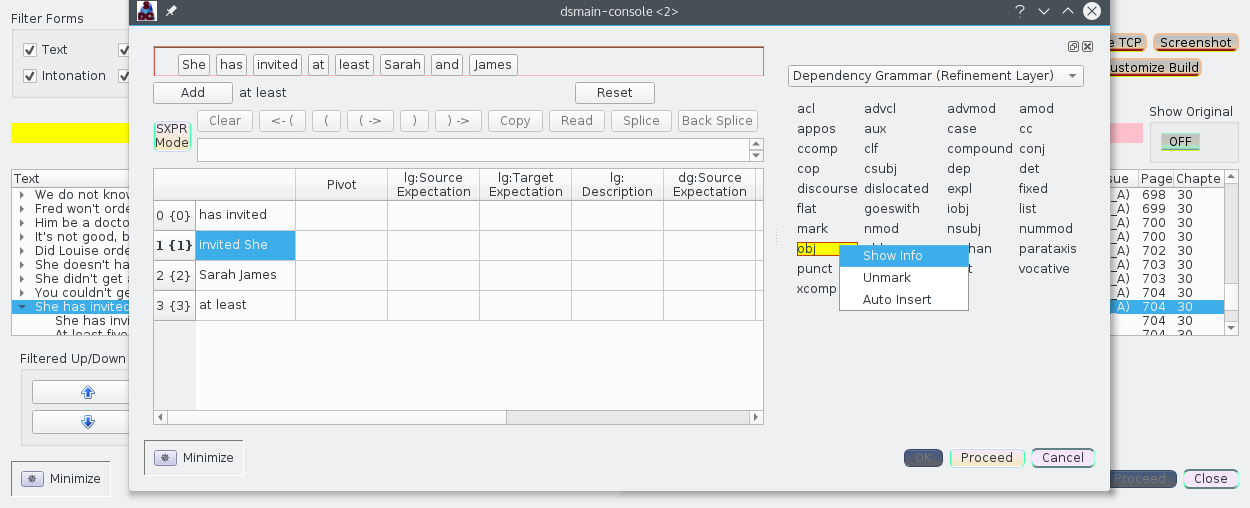
\includegraphics[scale=1]{texs/trilink.png}}
            
  \node [text width=7cm,inner sep=14pt,align=justify,%fill=logoCyan!20, draw=logoBlue, 
  draw opacity=0.9,line width=2mm, fill opacity=0.9,
  draw = logoCyan!50!brown,
  top color=brown!20,text=black,
  bottom color=logoCyan!2,
  rounded corners=6pt]
   at (0.41,0.39){\annfont\textbf{Users can select word-pairs 
   from samples being annotated and then identify 
   the relationship between the selected words, as understood 
   according to Link or Dependency Grammars.  The 
   list of link/dependency relations provides 
   an interface to research and read overviews about the 
   relationships.}};

\curicon{0.77}{0.48}


%\annotatedFigureBox{0.93,0.02}{0.985,0.945}{1}{0.985,0.945}%                
%\annotatedFigureBox{0.005,0.82}{0.43,0.98}{2}{0.43,0.82}%
%\annotatedFigureBox{0.01,0.1}{0.55,0.334}{3}{0.55,0.334}            
            
      %      \annotatedFigureBox{0.222,0.284}{0.3743,0.4934}{B}{0.3743,0.4934}%tr
      %      \annotatedFigureBox{0.555,0.784}{0.6815,0.874}{C}{0.555,0.784}%bl
      %      \annotatedFigureBox{0.557,0.322}{0.8985,0.5269}{D}{0.8985,0.5269}%tr
  

  
        \end{annotatedFigure}

\end{frame}
